\section{实验:用伏特表、安培表测电阻}\label{sec:8-8}

\begin{wrapfigure}{r}{7cm}
    \centering
    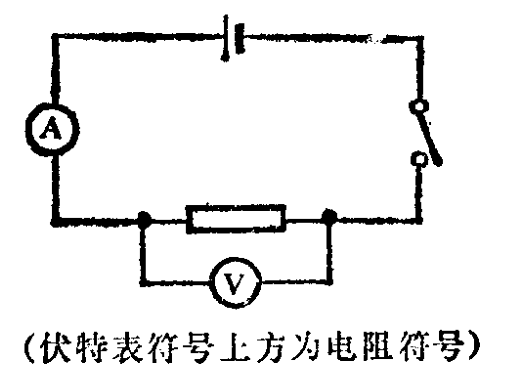
\includegraphics[width=6cm]{../pic/czwl2-ch8-18}
    \caption{}\label{fig:8-18}
\end{wrapfigure}

在这个实验里,我们将用伏安法测定一只碳膜电阻(或线绕电阻)的阻值。
从前面的例题 3 知道,只要测出电阻两端的电压 $U$ 和通过它的电流强度 $I$,就可以算出电阻值 $R$。
在这个实验里,除了待测电阻以外,还需要伏特表、安培表、电池、电键和几根导线。

选用实验器材的时候,不但要考虑需要用哪些器材,还需要考虑器材的规格和性能(如电源的电压值、电表的量程)。
例如,待测电阻的阻值很大,而电源电压不高,安培表可能显示不出电流值,就需要选用能测微弱电流的电流表。
在初中物理实验里,器材的规格已经由老师选定了,但我们还是应该在使用之前注意了解器材的规格。

照图 \ref{fig:8-18} 连接电路,闭合电键,记下电路中的电流强度和待测电阻两端的电压。
改变电池的个数,以改变加在待测电阻上的电压。
测出通过待测电阻的电流强度和它两端的电压,共记下三组电流强度和电压值。
根据每组数据,算出电阻值。
自己设计一个表格,把记下和算出的三组数据都填在表里。
最后求出电阻的平均值,作为待测电阻的阻值。

